\documentclass[../DS07.tex]{subfiles}
\graphicspath{{./figures/}}

% \subimport{/home/nora/Documents/Enseignement/Prepa/bpep/exercices/DS/satellite_autour_de_la_terre/}{sujet.tex}

\begin{document}
\exercice[50]{Satellite en orbite terrestre\ifcorrige{~\small\textit{(D'après
			TSI 2010)}}}

\subsection{Etude dynamique}

\enonce{
	On étudie le mouvement autour de la Terre d'un satellite $S$ de masse $m$
	placé dans le champ gravitationnel terrestre. On néglige les frottements.
}

\QR[5]{%
	Définissez les référentiels terrestres et géocentrique. Dans quel référentiel
	faut-il se placer pour cette étude~?
}{%
	Le référentiel géocentrique est lié au repère dont le centre est le centre de
	masse \pt{1} de la Terre et dont les axes pointent vers trois étoiles fixes
	lointaines. \pt{1}
	\smallbreak
	Un référentiel terrestre est lié au repère dont le centre est un point à la
	surface de la Terre \pt{1} et dont les axes sont solidaires à la Terre, donc
	en rotation par rapport à l'axe des pôles fixe \pt{1} dans le référentiel
	géocentrique.
	\smallbreak
	On étudie le mouvement du satellite dans le référentiel géocentrique supposé
	galiléen. \pt{1}
}

\QR[4]{%%
	Déterminer l'expression de la force $\Ff$ à laquelle le satellite $S$ est
	soumis. On exprimera $\Ff$ en fonction de $m$, $\Gc $, $M_T$, $r$
	et d'un vecteur unitaire que l'on précisera.
	\smallbreak
	Déterminer de même l'expression de la force $\Ff'$ à laquelle la Terre est
	soumise de la part du satellite. Justifier.
}{%
	\ifstudent{
		\smallbreak
		\vspace{-25pt}
	}
	\begin{isd}[interior hidden]
		La force d'interaction gravitationnelle exercée par la Terre sur le satellite
		est
		\[
			\boxed{\Ff \stm{=} -\frac{\Gc mM_T}{r^2}\er}
		\]
		où $\er$ est le vecteur unitaire dirigé du centre de la Terre $O$ vers
		le centre du satellite $M$. \pt{1}
		\tcblower
		D'après le principe des actions réciproques (troisième loi de \bsc{Newton} \pt{1}),
		on a~:
		\[
			\boxed{\Ff' \stm{=} -\Ff =\frac{\Gc mM_T}{r^2}\er}
		\]
	\end{isd}
	\vspace{-15pt}
}

\QR[7]{%
	Montrer que le mouvement est nécessairement plan. Sachant qu'à l'instant $t=0$
	le satellite se trouve au point $\Mr_0$ et a une vitesse $v_0$, préciser le
	plan dans lequel se fait le mouvement.
}{%
	On se place dans le référentiel géocentrique. La seule force exercée par le
	satellite est la force $\Ff$. \pt{1} Elle est centrale de centre $O$, ainsi, son
	moment par rapport à $O$ est nul~:
	$\Mcf_{\Or}(\Ff) \stm{=} \OM\wedge \Ff \stm[-1]{=} \of$.
	\smallbreak
	D'après le théorème du moment cinétique par rapport au point $O$, on a
	\begin{gather*}
		\dv{\Lcf_{\Or}(\Mr)}{t} \stm{=} \Mcf _{\Or}(\Ff )=\of
		\Lra
		\Lcf_{\Or}(\Mr) \stm{=} \vcte = \Lc_0 \uz
		\\\Ra
		\OM(t)\wedge m\vf_{\Mr}(t) \stm{=} \Lc_0 \uz = \OM(0) \wedge m\vf_{\Mr}(0)
	\end{gather*}
	avec $\uz$ la direction initiale du moment cinétique. Ainsi, le vecteur $\OM$
	reste constamment perpendiculaire à un vecteur constant, donc le mouvement est
	plan et le plan du mouvement passe par le centre de force $O$. En
	l'occurrence, le plan est $(\Or,\vvr{OM_0}, \vv{v_0})$. \pt{1}
}

\enonce{
	Dans la suite de cette partie, on se placera dans le cas d'une
	trajectoire \underline{circulaire} de rayon $r$ et d'altitude $h$ autour de la
	Terre (avec $r=R_T+h$) et on utilisera les coordonnées cylindriques.
	\smallbreak
	L'espace est rapporté à la base cylindrique $(\er, \et, \ez)$, un point
	quelconque de l'espace étant repéré par ses coordonnées ($r, \th, z$).
	\smallbreak
	Le plan dans lequel se fait le mouvement du satellite est le plan du repère
	cylindrique contenant l'origine $O$ du repère (le point $O$ étant le centre de
	la Terre) et les vecteurs $(\er, \et)$.
}

\QR[4]{%
	Montrer que la norme $v$ de la vitesse du satellite $S$ est nécessairement
	constant au cours du mouvement et déterminer son expression en fonction de
	$\Gc $, $M_T$ et $r$.
}{%
	\[
		\OM=r\er
		\qquad
		\vf =r\tp\et
		\qquad
		\af =-r\tp^2\er+r\tpp\et
		\qquad \pt{1}
	\]
	D'après le PFD appliqué au satellite dans le référentiel géocentrique supposé
	galiléen, on a~:
	\begin{gather*}
		m\af \stm{=} \Ff
		\Rightarrow
		-mr\tp^2\er+rm\tpp\et = -\frac{\Gc mM_T}{r^2}\er
		\\\beforetext{Sur $\et \Ra $}
		\tpp=0 \Rightarrow \tp=\text{cte}
		\tag*{donc $\norm{\vf} = \abs{r\tp}$ uniforme \pt{1}}
		\\\beforetext{Sur $\er \Ra $}
		mr\tp^2 = \frac{\Gc mM_T}{r^2}
		\Rightarrow
		r\frac{v^2}{r^2} = \frac{\Gc M_T}{r^2}
		\Rightarrow
		\boxed{v \stm{=} \sqrt{\frac{\Gc M_T}{r}}}
	\end{gather*}
}

\QR[2]{%
	Déterminer l'expression de la période $T$ du mouvement de rotation de $S$
	autour de la Terre en fonction de $v$ et $r$ puis en fonction de
	$\Gc $, $M_T$ et $r$. En déduire la troisième loi de \bsc{Kepler}.
}{%
	On a
	\[
		T \stm{=} \frac{2\pi r}{v} =
		\frac{2\pi r}{\sqrt{\frac{\Gc M_T}{r}}} =
		2\pi\sqrt{\frac{r^3}{\Gc M_T}}
		\Leftrightarrow
		\boxed{\frac{T^2}{r^3} \stm{=} \frac{4\pi^2}{\Gc M_T}}
	\]
	ce qui correspond à la traduction mathématique de la troisième loi énoncée par
	\bsc{Kepler}.
}

\QR[3]{%
	Indiquer une méthode pour déterminer la masse de la Terre. Donner alors un
	ordre de grandeur de la masse de la Terre à partir de vos connaissances
	astronomiques.
}{%
	On peut, à partir de la trajectoire d'un satellite naturel ou artificiel
	connaître $r$ et $T$, on en déduit alors $M_T$ en utilisant la 3ème loi de
	\bsc{Kepler} \pt{1}. Mieux, on peut relever $r$ et $T$ pour différent
	satellites, et tracer $T^2$ en fonction de $r^3$. On obtient alors une droite
	de pente $\frac{4\pi^2}{\Gc M_T}$, ce qui permet d'en déduire $M_T$ (en
	supposant $\Gc$ connu~!).
	\smallbreak
	Pour le cas de la lune~: $T=\SI{28}{jours}$ et $r=\SI{384e6}{m}$ \pt{1}. On en
	déduit la masse de la Terre~: $\xul{M_T=\SI{6.10e24}{kg}}$.~\pt{1}
}

\QR[3]{%
	Un autre satellite $S'$ de masse $m'$ en orbite circulaire autour de la Terre
	a une trajectoire de rayon $r$ égal au rayon de la trajectoire de $S$. Les
	deux satellites tournent dans le même plan. $S$ et $S'$ risquent-ils de se
	heurter au cours du mouvement~? On justifiera la réponse apportée.
}{%
	Si les deux satellites sont à la même distance de la terre, ils ont la même
	vitesse. \pt{1} Si de plus ils sont dans un même plan, alors ils ont des
	trajectoires identiques, \pt{1} parcourues à la même vitesse~: ils ne peuvent
	pas se heurter (sauf si leurs vitesses sont opposées). \pt{1}
}

\subsection{Étude énergétique}

\enonce{
	La force à laquelle le satellite $S$ est soumis dérive d'une énergie
	potentielle $\Ec_p$ telle que $\Ec_p$ peut s'écrire sous la forme
	$\Ec_p=-\frac{k}{r}$ avec $k$ une constante positive. On prendra par
	convention une énergie potentielle nulle à l'infini.
	\smallbreak
	On ne se limitera pas, dans cette partie, à un mouvement circulaire, mais on
	se placera dans le cas d'un mouvement quelconque du satellite $S$ autour de la
	Terre.
	\smallbreak
	On note $C$ la constante des aires définie par $C=r^2\tp$.
}

\QR[4]{%
	Déterminer l'expression de $k$ en fonction des données du problème en
	établissant l'expression de $\Ec_p$.
}{%
	\[
		\delta W \stm{=} \Ff \cdot \dd \OM =
		-\frac{\Gc M_Tm}{r^2}\er\cdot (\dd r\er + r \stm{\dd{\th}}\et + \dd{z}\ez) =
		-\frac{\Gc M_Tm}{r^2}\dd r =
		-\dd \pa{\frac{\Gc M_Tm}{r}+C}
	\]
	Ainsi, le travail élémentaire de la force $\Ff$ peut se mettre sous la
	forme $-\dd \Ec_p$, donc elle est conservative et dérive de l'énergie
	$\DS\Ec_p(r) \stm{=} -\frac{\Gc M_Tm}{r}+C$. En choisissant $Ep(+\infty) \stm{=} 0$, on a
	$C=0$, et on en déduit
	\[
		\Ec_p(r)=-\frac{k}{r}
		\qav
		\boxed{k \stm{=} \Gc M_Tm}
	\]
}

\QR[10]{%
	Déterminer l'expression de l'énergie mécanique $\Ec_m$ du satellite $S$ en
	fonction de $m$, $r$, $\rp$, $\tp$ et $k$. En déduire
	l'expression de l'énergie potentielle effective du satellite en fonction de
	$m$, $C$, $r$ et $k$.
	\smallbreak
	Donner l'allure de la représentation graphique de l'énergie potentielle
	effective en fonction de $r$ en justifiant les limites. Quelles sont les
	régions accessibles sur un diagramme en énergie potentielle~?
	\smallbreak
	En exploitant cette courbe, indiquer en fonction de la valeur de l'énergie
	mécanique le type de trajectoire suivie par le satellite et préciser dans
	chaque cas s'il s'agit d'un état de diffusion ou d'un état lié.
}{%
	\ifstudent{
		\smallbreak
		\vspace{-40pt}
	}
	\begin{isd}[interior hidden]
		\begin{align*}
			\dv{\Ec_m}{t} \overset{\rm TEM}{=} 0
			\quad       & \text{et} \quad
			\Ec_m = \Ec_c + \Ec_p \quad \pt{1}
			\\
			\beforetext{Or}
			\OM = r \er & \Ra \vf = \rp \er+ r \tp \et
			\\\Ra
			v^2   \stm{=} \rp^2 + (r\tp)^2
			            & \Ra
			\Ec_m = \frac{1}{2}m\rp^2 +
			\underbracket{\frac{1}{2}mr^2\tp^2 + -\frac{k}{r}}_{\Ec_{p,\rm eff}}
		\end{align*}
		\tcblower
		or $\boxed{\tp = C/r^2}$ d'où
		\begin{gather*}
			\boxed{\Ec_{p, \rm eff}(r)\stm{=}\frac{1}{2}m\frac{C^2}{r^2}-\frac{k}{r}}
		\end{gather*}
	\end{isd}
	\noindent
	\begin{minipage}[c]{.40\linewidth}
		\begin{center}
			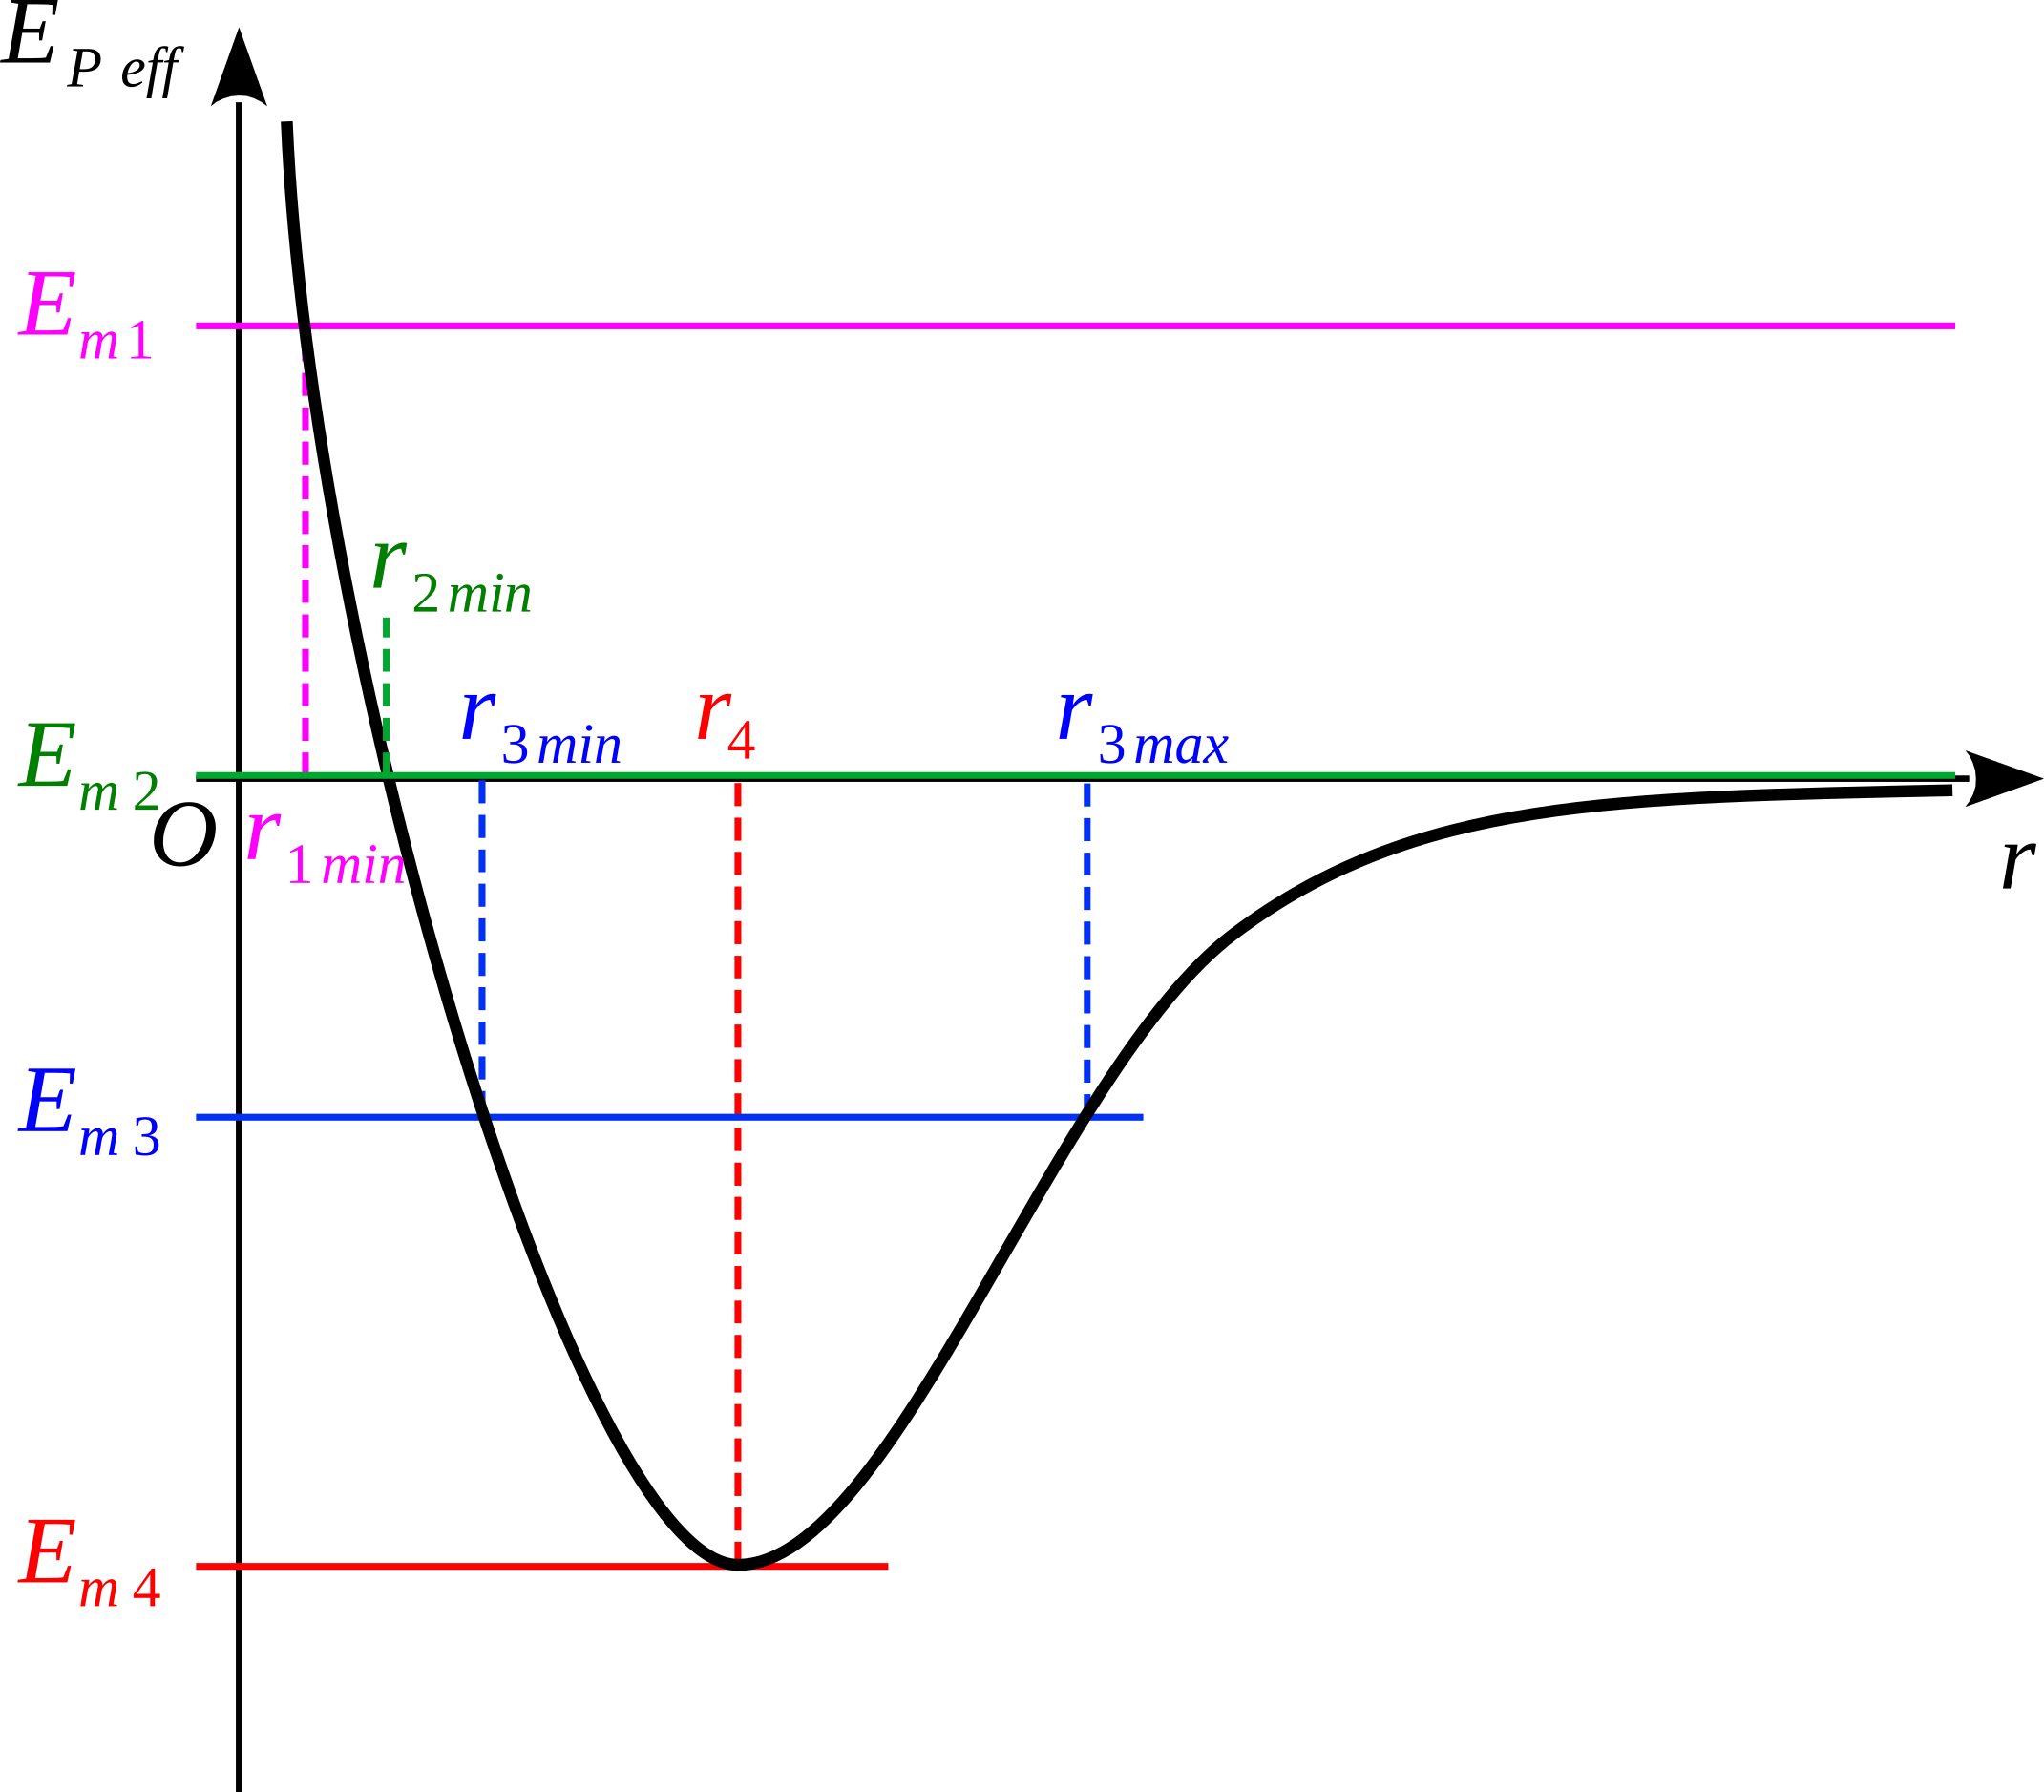
\includegraphics[width=.9\linewidth]{ep_eff-att_color.png}
			\captionof{figure}{Graphique de $\Ec_{p,\rm eff}(r)$\protect\pt{2}}
		\end{center}
	\end{minipage}
	\hfill
	\begin{minipage}[c]{.55\linewidth}
		\begin{itemize}
			\item $\Ec_{p, \rm eff}(r) \Sim_{r \to 0} \frac{1}{2}m\frac{C^2}{r^2}$,
			      et tend donc vers $±\infty$. \pt{1}
			\item $\Ec_{p, \rm eff}(r) \Sim_{r \to + \infty} -\frac{k}{r}$, et
			      tend donc vers $0^-$ (donc par valeurs négatives). \pt{1}
			\item De plus, $\Ec_m = \cte = \frac{1}{2}m\rp^2+\Ec_{p, \rm eff}(r) > \Ec_{p,
					      \rm eff}$, donc les régions accessibles sont celles pour lesquelles
			      $\boxed{\Ec_{p, \rm eff}(r)<\Ec_m}$. \pt{1}
		\end{itemize}
	\end{minipage}
	\smallbreak
	On en déduit donc~: \pt{2}
	\begin{itemize}
		\item Si $\Ec_{m}<\Ec_{m,4}$, aucun mouvement n'est possible
		\item Si $\Ec_m=\Ec_{m,4}$, alors $r=r_{4}$ est constant~: la trajectoire est
		      circulaire (état lié)
		\item Si $\Ec_{m_4}<\Ec_m<\Ec_{m,2} = 0$, $r$ est compris entre 2 valeurs $r_{3,min}$ et
		      $r_{3,max}$~: mouvement elliptique (état lié)
		\item Si $\Ec_m=\Ec_{m,2} = 0$, le satellite peut partir à l'infini mais sa vitesse à
		      l'infini est nulle~: le mouvement est parabolique (état de diffusion)
		\item Si $\Ec_m>0$~: le mouvement est hyperbolique (état de diffusion)
	\end{itemize}
}

\QR[5]{%
	Déterminer l'énergie mécanique $\Ec_{m}$ associée à une trajectoire circulaire
	de rayon $r_c$ en fonction de $r_c$, $m$, $\Gc$ et $M_T$. Définir puis
	déterminer la première vitesse cosmique $v_1$ par une rapide étude
	énergétique, fonction de $R_T$, $\Gc$ et $M_T$.
}{%
	\vspace{-15pt}
	\begin{gather*}
		\Ec_m=\frac{1}{2}mv^2-\frac{\Gc M_Tm}{r_c}
		\\\beforetext{Or, $v=\sqrt{\frac{\Gc M_T}{r_c}} \Ra $}
		\Ec_m =
		\frac{1}{2}\frac{\Gc M_Tm}{r_c}-\frac{\Gc M_Tm}{r_c}
		\Lra
		\boxed{\Ec_m \stm{=} -\frac{1}{2}\frac{\Gc M_Tm}{r_c} }
	\end{gather*}
	La première vitesse cosmique, ou \textit{vitesse de satellisation minimale},
	est la \textbf{vitesse minimale} à fournir à un objet situé sur Terre pour
	pouvoir le placer en orbite \textbf{circulaire} autour de la Terre, à un rayon
	$R_T$~: \pt{1}
	\begin{gather*}
		\Ec_{m,\rm sol} \stm{=} \frac{1}{2}mv_c{}^2 -\Gc \frac{mM_\Ter}{R_\Ter}
		\qet
		\Ec_{m,\rm cercle} \stm{=} -\Gc \frac{mM_\Ter}{2R_\Ter}
		\\
		\beforetext{Or système conservatif après le lancer $\Ra$}
		\frac{1}{2}mv_c{}^2 -\Gc \frac{mM_\Ter}{R_\Ter} =
		-\Gc \frac{mM_\Ter}{2R_\Ter}
		\\\Lra
		\boxed{v_c \stm{=} \sqrt{\frac{\Gc m_\Ter}{R_\Ter}}}
	\end{gather*}
}
\end{document}
